\documentclass[12pt,letterpaper]{article}
\usepackage{fullpage}
\usepackage[top=2cm, bottom=4.5cm, left=2.5cm, right=2.5cm]{geometry}
\usepackage{amsmath,amsthm,amsfonts,amssymb,amscd}
\usepackage{lastpage}
\usepackage{enumerate}
\usepackage{fancyhdr}
\usepackage{mathrsfs}
\usepackage{xcolor}
\usepackage{graphicx}
\usepackage{hyperref}
\usepackage{tikz}
\usepackage{enumitem}
\usepackage{braket}
\usepackage{tkz-euclide}

\hypersetup{%
  colorlinks=true,
  linkcolor=blue,
  linkbordercolor={0 0 1}
}

\setlength{\parindent}{0.0in}
\setlength{\parskip}{0.05in}

% Edit these as appropriate
\newcommand\course{}
\newcommand\hwnumber{5}                  % <-- homework number
\newcommand\NetIDa{Ivan Zhytkevych}
% \newcommand\NetIDb{Ivan Zhytkevych}

\pagestyle{fancyplain}
\headheight 35pt
\lhead{\NetIDa}
% \lhead{\NetIDa\\\NetIDb}                 % <-- Comment this line out for problem sets (make sure you are person #1)
\chead{\textbf{\Large Homework \hwnumber}}
\rhead{\course \\ \today}
\lfoot{}
\cfoot{}
\rfoot{\small\thepage}
\headsep 1.5em



\begin{document}


\section*{Problem 5.15}

\[ \Omega = \{\text{cards}\}; \; |\Omega| = 52 \]

\begin{itemize}

    \item[a.]
        \[ A = \{ \text{hearts} \}; \; |A| = 13 \]
        \[ B = \{ \text{red cards} \}; \; |B| = 26  \]
        \[ P(A | B) = \frac{P(A\cap B)}{B} = \frac{1}{2} \]

    \item[b.]
        \[ A = \{\text{ rank 11, 12, 13, 14 } \}; \; \]
        \[ B = \{ hearts \}; \]
        \[ P(A|B) = \frac{4}{13} \]


    \item[c.]
        \[ P(A|B) = \frac{2}{26} = \frac{1}{13} \]


\end{itemize}

%%%%%%%%%%%%%%%%%%%%%%%%%%%%%%%%%%%%%%%%%%%%%%%%%%%%%%%%%%%%%%%%%%%%%%%%%%%%%%%

\section*{Problem 5.16}

\[ \Omega = \{ (i, j) \mid i, j \in \{1,2,3,4,5,6\} \}; \; |\Omega| = 36 \]
\[ A = \set{ (i, j) \in \Omega  \mid i + j > 7 } ;\; |A| = 5 + 4 + 3 + 2 + 1 = 15 \]

\begin{itemize}

    \item[a] 
        \[ B = \{ (i,j) \in \Omega | i = 1 \} ;\; |B| = 6  \]
        \[ A \cap B = \emptyset \]
        \[ P(A|B) = 0 \]

    \item[b]
        \[ B = \set{ (i,j) \in \Omega \mid i < 5 }; \; |B| = 4 \cdot 6 = 24  \]
        \[ |A \cap B| = 6 \]
        \[ P(A|B) = \frac{1}{4} \]

\end{itemize}

%%%%%%%%%%%%%%%%%%%%%%%%%%%%%%%%%%%%%%%%%%%%%%%%%%%%%%%%%%%%%%%%%%%%%%%%%%%%%%%%%%%%%

\section*{Problem 5.17}

\[ \Omega = \set{ (i,j) \mid i,j \in \set{0,1}, \text{0 - tails, 1 - heads} } \]
\[ A = \set{(1,j) \mid j \in \set{0, 1}} \]
\[ B = \set{ (i, 1) \mid i \in \set{0, 1} } \]
\[ C = \set{ (i, j) \in \Omega \mid i = j) } \]
\[ P(A) = 1/2 \]
\[ P(B) = 1/2 \]
\[ P(C) = 1/2 \]
\[ P(A \cap B) = \frac{1}{4} = P(A)P(B) \]
\[ P(B \cap C) = \frac{1}{4} = P(B)P(C) \]
\[ P(A \cap C) = \frac{1}{4} = P(A)P(C) \]
\[ P(A \cap B \cap C) = P(\set{(1,1)}) = \frac{1}{4} \neq \frac{1}{8} = P(A)P(B)P(C) \]

%%%%%%%%%%%%%%%%%%%%%%%%%%%%%%%%%%%%%%%%%%%%%%%%%%%%%%%%%%%%%%%%%%%%%%%%%%%%%%%

\section*{Problem 5.18}

\[ \Omega = \set{ \set{i,j,k} \mid i,j,k \in \mathbb{N}, i,j,k \in [1,10], i \neq j \neq k } \]
\[ |\Omega| = C_{10}^{3} = \frac{10!}{3! 7!} = 4 \cdot 3 \cdot 10 \]
\[ B = \set{ \set{i,j,k} \in \Omega \mid i \in [8,10] \text{ or } j \in [8,10] \text{ or } k \in [8,10] } \]
\[ A = \set{ \set{i,j,k} \in \Omega \mid \exists a, b \in \set{i,j,k} : a,b \in [1,7] } \]

\[ A \cap B = \set{ \set{i,j,k} \in \Omega \mid \text{two white, one black} } \]
\[ P(B) = 1 - P(\overline B) = 1 - \frac{|\overline B|}{|\Omega|} = 1 - \frac{C_7^3}{10 \cdot 4 \cdot 3}
= 1 - \frac{7!}{3! \cdot 4! \cdot 10 \cdot 4 \cdot 3}= \]
\[ = 1 - \frac{5 \cdot 6 \cdot 7}{ 2 \cdot 3 \cdot 10 \cdot 4 \cdot 3} = 1 - \frac{7}{24} =
\frac{17}{24} \]

\[ |A \cap B| = C_{7}^2 C_3^1 = \frac{7!}{2!5!} 3 = \frac{7 \cdot 6}{2} 3 = 7 \cdot 9  \]
\[ P(AB) = \frac{7 \cdot 9}{10 \cdot 4 \cdot 3} = \frac{21}{40} \]
\[ P(A|B) = \frac{21 \cdot 24}{40 \cdot 17} = \frac{63}{85} \]


%%%%%%%%%%%%%%%%%%%%%%%%%%%%%%%%%%%%%%%%%%%%%%%%%%%%%%%%%%%%%%%%%%%%%%%%%%%%%%%

\section*{Problem 5.19}

\[ \Omega = \set{ (\zeta_1, \zeta_2) \in [0,1]^2 } \]
\[ B = \set{ (\zeta_1, \zeta_2) \in \Omega \mid \zeta_1 + \zeta_2 \leq 1 } \]

\begin{center}
    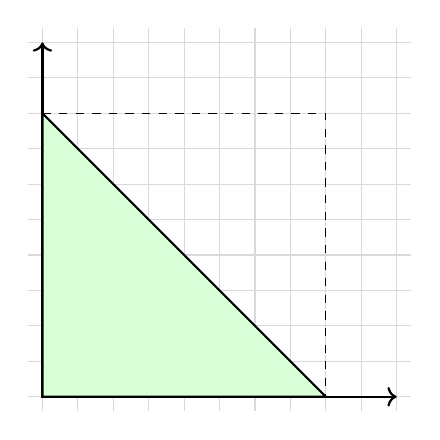
\begin{tikzpicture}[scale=0.9]
        \draw[step=0.5, gray!30, thin, xshift=0cm, yshift=0cm] (-0.2, -0.2) grid (5.2,5.2);
        \draw[thick, <->] (0, 5) 
            -- (0, 0) 
            -- (5, 0) ;

        \draw[dashed] (0, 4) -| (4, 0);

        \draw[fill=green!15, thick] (0, 4) -- (4, 0) -- (0, 0) -- cycle;
    \end{tikzpicture}
\end{center}


\begin{itemize}

    \item[a]
        \[ A = \set{ (\zeta_1, \zeta_2) \in \Omega \mid | \zeta_1 - \zeta_2 | < 1 } \]

        \begin{center}
            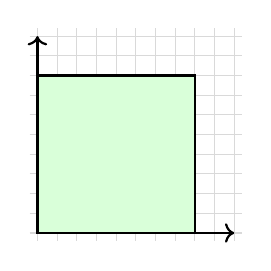
\begin{tikzpicture}[scale=0.5]
                \draw[step=0.5, gray!30, thin, xshift=0cm, yshift=0cm] (-0.2, -0.2) grid (5.2,5.2);
                \draw[thick, <->] (0, 5)
                    -- (0, 0) 
                    -- (5, 0);

                \draw[dashed] (0, 4) -| (4, 0);

                \draw[fill=green!15, thick] (0, 4) -- (4, 4) -- (4, 0) -- (0, 0) -- cycle;
            \end{tikzpicture}
        \end{center}

        \[ P(A|B) = \frac{P(B)}{P(B)} = 1 \]

    \item[b]
        \[ A = \set{ (\zeta_1, \zeta_2) \in \Omega \mid \zeta_1 \cdot \zeta_2 < \frac{1}{2} } \]
        \[  \zeta_2 < \frac{1}{2\zeta_1} \]

        \[ A \cap B = B \]
        \[ P(A|B) = 1 \]

    \item[c]
        \[ A = \set{ max(\zeta_1, \zeta_2) < 1/2 } \]
        \begin{center}
            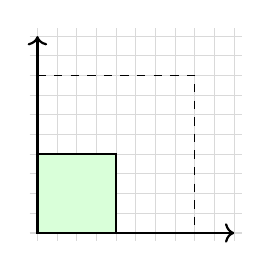
\begin{tikzpicture}[scale=0.5]
                \draw[step=0.5, gray!30, thin, xshift=0cm, yshift=0cm] (-0.2, -0.2) grid (5.2,5.2);
                \draw[thick, <->] (0, 5) 
                    -- (0, 0)
                    -- (5, 0) ;

                \draw[dashed] (0, 4) -| (4, 0);

                \draw[fill=green!15, thick] (0, 2) -- (2, 2) -- (2, 0) -- (0, 0) -- cycle;
            \end{tikzpicture}
        \end{center}

        \[ A \cap B = A \]
        \[ P(B) = \frac{1}{2} \]
        \[ P(A) = \frac{1}{4} \]
        \[ P(A|B) = \frac{1}{2} \]

    \item[d]
        \[ A = \set{ \zeta_1^2 + \zeta_2^2 < \frac{1}{4} } \]

        \[ A \cap B = A \]
        \[ P(A) = \frac{\pi \frac{1}{4}}{4} = \frac{\pi}{16} \]
        \[ P(A|B) = \frac{\pi}{16} \cdot \frac{2}{1} = \frac{\pi}{8} \]

    \item[e]
        \[ A = \set{ \zeta_1 > \zeta_2 } \]

        \begin{center}
            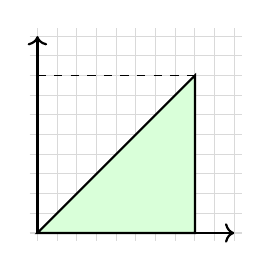
\begin{tikzpicture}[scale=0.5]
                \draw[step=0.5, gray!30, thin, xshift=0cm, yshift=0cm] (-0.2, -0.2) grid (5.2,5.2);
                \draw[thick, <->] (0, 5) 
                    -- (0, 0)
                    -- (5, 0) ;

                \draw[dashed] (0, 4) -| (4, 0);

                \draw[fill=green!15, thick] (0, 0) -- (4, 4) -- (4, 0) -- cycle;
            \end{tikzpicture}
        \end{center}
        \[ P(A|B) = \frac{1/4}{1/2} = \frac{1}{2} \]

\end{itemize}

%%%%%%%%%%%%%%%%%%%%%%%%%%%%%%%%%%%%%%%%%%%%%%%%%%%%%%%%%%%%%%%%%%%%%%%%%%%%%%%%%%%%

\section*{Problem 5.20}

\[ \Omega = \set{ (\varepsilon_1, \dots, \varepsilon_n) \mid \varepsilon_i \in \set{0,1}, \text{1 -
heads, 0 - tails} }; \; |\Omega| = 2^n \]
\[ A = \set{ (\varepsilon_1, \dots, \varepsilon_n) \in \Omega \mid \varepsilon_1 = 1 } \]
\[ B_k = \set{  (\varepsilon_1, \dots, \varepsilon_n) \in \Omega \mid \sum \varepsilon_i = k } \]
\[ P(A) = p \]
\[ P(B_k) = C_n^k p^k \cdot (1 - p)^{n-k} \]
\[ P(A B_k) = p (C_{n-1}^{k-1} p^{k-1} \cdot (1 - p)^{n-k}) \]
\[ P(A B_k) = P(A)P(B_k) \]
\[ p^k \frac{(n-1)!}{(k-1)! (n-k)!} (1-p)^{n-k} = p^{k+1} \frac{n!}{k! (n-k)!} (1-p)^{n-k} \]
\[ \frac{k}{n} = p \Rightarrow k = pn \]

%%%%%%%%%%%%%%%%%%%%%%%%%%%%%%%%%%%%%%%%%%%%%%%%%%%%%%%%%%%%%%%%%%%%%%%%%%%%%%%%%%%

\section*{Problem 5.21}

\[ \Omega = \left\{
        \begin{pmatrix}
            1 & 2 & 3 & \dots & 10 \\
            k_1 & k_2 & k_3 & \dots & k_{10}
        \end{pmatrix} \mid 
        k_i \in \set{ 1, \dots, 10 }
\right\} \]
\[ A = \left\{
        \begin{pmatrix}
            1 & 2 & 3 & 4 & 5 & \dots & 10 \\
            k_1 & k_2 & k_3 & 4 & k_5 & \dots & k_{10}
        \end{pmatrix} \in \Omega 
\right\} \]
\[ B = \left\{
        \begin{pmatrix}
            1 & 2 & 3 & \dots & 10 \\
            k_1 & k_2 & k_3 & \dots & k_{10}
        \end{pmatrix} \in \Omega \mid
        k_{2n} = 1, 2, 3, \; k_{2(n+1)} = 2, 3, 1, \; k_{2(n+2)} = 3, 1, 2
\right\} \]
\[ |B| = 3 \cdot 3! \cdot 7! \]
\[ A \cap B = \left\{
        \begin{pmatrix}
            1 & 2 & 3 & 4 & \dots & 10 \\
            k_1 & k_2 & k_3 & 4 & \dots & k_10
        \end{pmatrix} \in \Omega \mid
        k_6 = 1, 2, 3, \; k_8 = 2, 3, 1, \; k_10 = 3, 1, 2
\right\} \]
\[ |A \cap B| = 3! \cdot 6! \]
\[ P(A|B) = \frac{P(A \cap B)}{P(B)} = \frac{3! \cdot 6!}{ 3 \cdot 3! \cdot 7!} = \frac{1}{3 \cdot
7} = \frac{1}{21} \]

%%%%%%%%%%%%%%%%%%%%%%%%%%%%%%%%%%%%%%%%%%%%%%%%%%%%%%%%%%%%%%%%%%%%%%%%%%%%%%%%
\section*{Problem 5.22}
\[ \Omega = \left\{
        (\varepsilon_1, \dots, \varepsilon_7) \mid
        \varepsilon_i \in \set{0, 1}
\right\} \]
\[ A_i = \left\{
        (\varepsilon_1, \dots, \varepsilon_7) \in \Omega \mid
        \varepsilon_i = 1
\right\} \]
\[ \overline{A_i} = \left\{
        (\varepsilon_1, \dots, \varepsilon_7) \in \Omega \mid
        \varepsilon_i = 0
\right\} \]
\[ P(A_i) = C_{7}^{1} 0.1 \Rightarrow P(\overline{A_i}) = C_{7}^{1} 0.9 \]
\[ P(\mathcal{A}_j) = [ \text{probability of attack j times} ] = \] 
\[ = P( A_{a}^{C_a} \cap  A_{b}^{C_b} \cap A_{c}^{C_c} \cap A_{d}^{C_d} \cap A_{e}^{C_e} \cap A_{f}^{C_f}
\cap A_{g}^{C_g} ) = C_{7}^{j} 0.1 ^ {j} \cdot 0.9^{7-j} \]
\[ \sum C_k = i, \;\; A_{l}^{C_l} = \begin{cases}
    A_l, \; C_k = 1 \\
    \overline{A_l}, \; C_k = 0
\end{cases}
\]
\[ P(\mathcal{A}_2) = C_{7}^{2} 0.1^2 \cdot 0.9^5 \approx 0.124 \]
\[ P(\mathcal{A}_0) = 0.9^7 \approx 0.478 \]
\[ P(\mathcal{A}_0) + P(\mathcal{A}_1) + P(\mathcal{A}_2) = C_{7}^{0} 0.9^7 + C_{7}^{1}
    0.1\cdot0.9^6 + C_{7}^{2} 0.1^2 \cdot
0.9^5 \approx 0.478 + 0.372 + 0.124 = 0.974 \]

%%%%%%%%%%%%%%%%%%%%%%%%%%%%%%%%%%%%%%%%%%%%%%%%%%%%%%%%%%%%%%%%%%%%%%%%%%%%%%%%%%%

\section*{Problem 5.23}

$A_j$ - the coin is in $j$ box.
$B_i$ - you haven't found for a coin in $i$ box

\[ P(B_i|A_j) = \begin{cases}
    (1 - a_i), \;\; i = j \\
    1, \;\; i \neq j
\end{cases}
\]

\[ P(B_i|A_j) = \frac{P(B_i A_j)}{P(A_j)} = \frac{P(B_i A_j)}{P(B_i)} = P(A_j|B_i) \]
\[ P(B_i|A_j)P(A_j) = P(A_j|B_i)P(B_i) \]
\[ P(A_j|B_i) = \frac{P(B_i|A_j)P(A_j)}{P(B_i)} \]

\[ P(B_i) = P(B_i|A_j)P(A_j) + P(B_i|\overline{A_j})P(\overline{A_j}) = (1-a_i)p_i + (1-p_i) =
    1 - a_i p_i \]

\[ P(A_j|B_i) = \begin{cases}
    \frac{(1 - a_i) p_i}{1 - a_i p_i} , \;\; i = j \\
    \frac{p_j}{1 - a_i p_i}, \;\; i \neq j
\end{cases}
 \]

%%%%%%%%%%%%%%%%%%%%%%%%%%%%%%%%%%%%%%%%%%%%%%%%%%%%%%%%%%%%%%%%%%%%%%%%%%%%%%%%%%%

\section*{Problem 5.24}

\[ P(A|B) = P(B|A) \]
\[ P(A \cup B) = 1 \]
\[ P(A \cap B) > 0 \]

\[ P(A|B) = \frac{P(A \cap B)}{P(B)} = \frac{P(A \cap B)}{P(A)} = P(B|A) \;
    \Rightarrow \; P(A) = P(B) \]
    \[ P(A \cup B) =  P(A) + P(B) - P(A \cap B) \]
    \[ 1 = 2 P(A) - P(A \cap B) \]
    \[ P(A) = \frac{1}{2} + \frac{1}{2} P(A \cap B) \; \Rightarrow \; P(A) > \frac{1}{2} \]


%%%%%%%%%%%%%%%%%%%%%%%%%%%%%%%%%%%%%%%%%%%%%%%%%%%%%%%%%%%%%%%%%%%%%%%%%%%%%%%%%%%

\section*{Problem 5.25}

\[ A \subset B \]
\[ P(A \cap B) = [ A \subset B ] = P(A) \]
\[ \Rightarrow P(A) = P(A)P(B) \]
\[  P(B) = 1 : P(A) = P(A)P(B) = P(A) \]
\[  P(A) = 0 : 0 = P(A) = P(A)P(B) = 0 \]


%%%%%%%%%%%%%%%%%%%%%%%%%%%%%%%%%%%%%%%%%%%%%%%%%%%%%%%%%%%%%%%%%%%%%%%%%%%%%%%%%%%

\section*{Problem 5.26}

\[ P(A_1 \dots A_n | C) = \frac{P(A_1 \dots A_n C)}{P(C)} \]
\[ P(A_1 | C) P(A_2 | A_1 C) \dots P(A_n | A_1 \dots A_{n-1} C) = \frac{P(A_1 C)}{P(C)}
    \cdot \frac{P(A_1 A_2 C)}{P(A_1 C)} \dots \frac{P(A_1 \dots A_{n-1} A_n C)}{P(A_1 \dots
    A_{n-1}C)} = 
\]
\[ = \frac{P(A_1 \dots A_{n-1} A_n C)}{P(C)}  \]


%%%%%%%%%%%%%%%%%%%%%%%%%%%%%%%%%%%%%%%%%%%%%%%%%%%%%%%%%%%%%%%%%%%%%%%%%%%%%%%%%%%

\section*{Problem 5.27}

\[ P(A) = \begin{cases}
    0 \\
    1
\end{cases}
\]

\begin{itemize}
    \item[1)]
        \[ [P(A) = 0] \]

        \[ P(A)P(B) = 0 \]
        \[ P(A \cap B) \leq P(A) \Rightarrow P(A \cap B) = 0 \]

    \item[2)]
        \[ [P(A) = 1] \]

        \[ P(A) P(B) = 1 \]
        \[ P(\overline A \cap B) = 0 \]
        \[ P(\overline A \cap B) = P(B) - P(A \cap B) \]
        \[ P(A \cap B) = P(B) = P(A) P(B) = 1 \]

\end{itemize}

%%%%%%%%%%%%%%%%%%%%%%%%%%%%%%%%%%%%%%%%%%%%%%%%%%%%%%%%%%%%%%%%%%%%%%%%%%%%%%%%%%%

\end{document}

